%%%%%%%%%%%%%%%%%%%%%%%%%%%%%%%%%%%%%%%%%%%%%%%%%%%%%%%%%%%%%%%%%
% Projeto de Extensão da disciplina de Matemática Discreta
% Sub-projeto do ProgramAuto
% Autores:
%     Prof. Dr. Ruben Carlo Benante
%     Nome do Aluno 1
%     Nome do Aluno 2
%
% Data: 2021-06-14
%
% Assunto: escrever uma linha de explicação
%%%%%%%%%%%%%%%%%%%%%%%%%%%%%%%%%%%%%%%%%%%%%%%%%%%%%%%%%%%%%%%%%


%%%%%%%%%%%%%%%%%%%%%%%%%%%%%%%%%%%%%%%%%%%%%%%%%%%%%%%%%%%%%%%%%
% Para gerar o PDF use uma das 2 opções abaixo:
%
% Opção 1: com makefile
%    $ make ext-matdiscreta-benante-sobrenome1-sobrenome2.pdf
%
% Opção 2: comandos diretos:
%    $ pdflatex pext-matdiscreta-benante-sobrenome1-sobrenome2.tex -o pext-matdiscreta-benante-sobrenome1-sobrenome2.pdf
%    $ bibtex biblio 
%    $ pdflatex pext-matdiscreta-benante-sobrenome1-sobrenome2.tex -o pext-matdiscreta-benante-sobrenome1-sobrenome2.pdf

% preambulo %%%%%%%%%%%%%%%%%%%%%%%%%%%%%%%%%%%%%%%%%%%%%%%%%%%%%%
\documentclass[a4paper,10pt]{article} %twocolumn
\usepackage[utf8]{inputenc} % letras acentuadas
\usepackage[portuguese]{babel} % tradução de títulos
\usepackage{algorithm} % ambiente para índice de algoritmos
\usepackage{algpseudocode} % fonte e estilo do algoritmo
\usepackage{graphicx}
% \usepackage{natbib}
%[noend]

\floatname{algorithm}{Algoritmo} % tradução da palavra algorítimo no ambiente de índice

% capa %%%%%%%%%%%%%%%%%%%%%%%%%%%%%%%%%%%%%%%%%%%%%%%%%%%%%%
\title{ProgramAuto: Biblioteca Ncurses}
\author{Ruben Carlo Benante \\ Alex Bruno Seabra \\ Adriano Jose Morais Barros Silva \\ Jose Roberto Lopes Gentile Almeida \\ Arlon Nata Alves Granja Delmondes \\ Victor Lucas Cavalcante Moreira \\ Joao Pedro Henderson Sarruf \\ Victor Machado De Araujo}

\begin{document}

\maketitle

% resumo %%%%%%%%%%%%%%%%%%%%%%%%%%%%%%%%%%%%%%%%%%%%%%%%%%%%%%
\begin{abstract}

\textbf{Assunto:} Ensino da Linguagem de Programação \texttt{C}.
Vamos abordar a biblioteca Ncurses e explicar o funcionamento do projeto de extensão.


% descrever em poucas palavras seu projeto aqui 

\textbf{Local:} Escola Politécnica de Pernambuco - UPE/POLI

\textbf{Órgão Financiador:} N/A

\textbf{Caracterização:} Projeto de Extensão requisito da disciplina de Matemática Discreta, sub-projeto integrante do Projeto \texttt{ProgramAuto}

% Este é o fim do resumo.

\end{abstract}


% artigo %%%%%%%%%%%%%%%%%%%%%%%%%%%%%%%%%%%%%%%%%%%%%%%%%%%%%%
% seção de introdução %%%%%%%%%%%%%%%%%%%%%%%%%%%%%%%%%%%%%%%%%%%%%%%%%%%%%%
\section{Introdução}

% Descrever melhor seu projeto aqui 
O projeto de extensão vai ser um minicurso sobre a biblioteca Ncurses em linguagem C.Neste curso serão abordadas algumas das principais funções dessa biblioteca bemcomo algumas de suas aplicações.


% seção de objetivos %%%%%%%%%%%%%%%%%%%%%%%%%%%%%%%%%%%%%%%%%%%%%%%%%%%%%%
\section{Objetivos}

\subsection{Objetivo Geral}

O projeto tem como objetivo contribuir no processo de ensino-aprendizagem do cidadão interessado em imergir nas linguagens de programação e novas tecnologias da indústria 4.0.


\subsection{Objetivos Específicos}


\begin{itemize}
 \item Proporcionar um melhor ensino sobre Ncurses para os alunos de informática.
 \item Democratizar aulas de Ncurse, em português,  no Youtube não só para a comunidade acadêmica mas também para a população externa.
\end{itemize}


% seção de justificativa %%%%%%%%%%%%%%%%%%%%%%%%%%%%%%%%%%%%%%%%%%%%%%%%%%%%%%
\section{Justificativa}
A razão da implementação desse projeto é buscar a democratização do conhecimento visto que existem poucos conteúdos em língua portuguesa no youtube sobre a biblioteca Ncurses.

%\begin{figure}[ht]
%\centering
%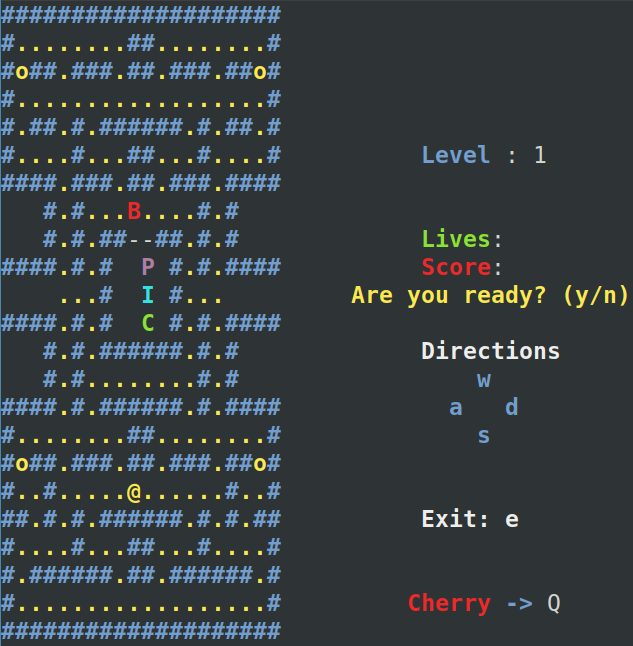
\includegraphics[width=.80\linewidth]{imagem.png}
%\caption{Exemplo de aplicação do Ncurses}
%\label{fig:xsort}
%\end{figure}


% seção de metodologia %%%%%%%%%%%%%%%%%%%%%%%%%%%%%%%%%%%%%%%%%%%%%%%%%%%%%%
\section{Metodologia}
 O método de pesquisa escolhido favorece uma liberdade na análise dos conceitos e teorias que serão abordadas, possibilitando assumir várias posições no decorrer dopercurso. 
 Para obter os resultados pretendidos, a equipe começará pela etapa da fundamentação teórica, onde serão levantados os principais conceitos sobre o tema, a fim de aprimorar e embasar todo trabalho.
 Em seguida, serão estruturados roteiros  que irão guiar cada integrante na elaboração das suas respectivas atividades.
 Ademais,  serão feitas reuniões periódicas e ajustes das ações em andamento e também  a elaboração de slides para auxiliar no processo de gravação das aulas.
 Outrossim, aulas serão ministradas e gravadas com o suporte de toda a  equipe e posteriormente organizadas em uma playlist dentro de um canal feito exclusivamente para o projeto no Youtube.
 Por fim, um relatório final será elaborado e entregue ao departamento responsável com o intuito de registrar e efetivar o trabalho desenvolvido pelos estudantes.

% subseção equipamentos %%%%%%%%%%%%%%%%%%%%%%%%%%%%%%%%%%%%%%%%%%%%%%%%%%%%%%
\subsection{Equipamentos Necessários}

%Listar os equipamentos necessários para a implementação do projeto.
\begin{itemize}
 \item Programas de edição de vídeos 
 \item Programas para a criação de slides
 \item Acesso a internet de qualidade
 \item Câmera ou webcam de qualidade
 \item Materiais em geral como: folhas, caneta, etc
 \item Computador e smartphones para cada integrante da equipe.
\end{itemize}

% subseção com algoritmo %%%%%%%%%%%%%%%%%%%%%%%%%%%%%%%%%%%%%%%%%%%%%%%%%%%%%%
\subsection{Implementação}
 A implementação será feita por meio da criação de uma playlist em um canal específico do projeto no Youtube e/ou plataforma escolhida pelo professor orientador do projeto.


% seção Plano de Trabalho %%%%%%%%%%%%%%%%%%%%%%%%%%%%%%%%%%%%%%%%%%%%%%%%%%%%%%
\section{Plano de Trabalho}

 \begin{itemize}
  \item Pesquisa do conteúdo 
  \item Implementação dos códigos que serão usados para exemplificação
  \item Roteiro dos vídeos
  \item Criação dos slides e dos vídeos
 % \item Editar os vídeos
%  \item Criação da playlist no canal no Youtube
%  \item Elaboração do relatório final
%  \item Entrega e validação do projeto pelo setor responsável
\end{itemize}

% seção Plano de Trabalho %%%%%%%%%%%%%%%%%%%%%%%%%%%%%%%%%%%%%%%%%%%%%%%%%%%%%%
\section{Cronograma}
Tabela contendo todas as informações acerca do planejamento do projeto bem como suas datas

\begin{table}
\begin{center}
 \caption{Tabela de cronograma do projeto de extensão}
\begin{tabular}{|l|r|}
  \hline \hline
  \textbf{Etapas} & \textbf{Datas} \\ \hline \hline
   Pesquisar o conteúdo & 24/06/ \\ \hline
   implementação dos códigos & 05/07/ \\ \hline
%   roteiro dos vídeos & 12/07/ \\ \hline
%   Criação dos slides e vídeos  & 19/07/ \\ \hline
%   Editar os vídeos  & 23/07/ \\ \hline
%   Criação da Playlist  & 30/08/ \\ \hline
   Elaboração do Relatório Final  & 01/09/ \\ \hline
   Entrega e validação & 16/09/2021 \\ \hline \hline
\end{tabular} 
\label{tab:resultados}
\end{center}
\end{table}


% seção de impactos alcançados %%%%%%%%%%%%%%%%%%%%%%%%%%%%%%%%%%%%%%%%%%%%%%%%%%%%%%
\section{Impactos e Transferências}

% subseção de impacto científico %%%%%%%%%%%%%%%%%%%%%%%%%%%%%%%%%%%%%%%%%%%%%%%%%%%%%%
\subsection{Impacto Científico}

Não há impacto científico relevante.

% subseção de impacto tecnológico %%%%%%%%%%%%%%%%%%%%%%%%%%%%%%%%%%%%%%%%%%%%%%%%%%%%%%
\subsection{Impacto Tecnológico}

Não há impacto tecnológico relevante.

% subseção de econônimo %%%%%%%%%%%%%%%%%%%%%%%%%%%%%%%%%%%%%%%%%%%%%%%%%%%%%%
\subsection{Impacto Econômico}

Não há impacto econômico relevante.

% subseção de impacto social %%%%%%%%%%%%%%%%%%%%%%%%%%%%%%%%%%%%%%%%%%%%%%%%%%%%%%
\subsection{Impacto Social}

O projeto visa contribuir com a sociedade transmitindo conhecimento gratuito aberto a todas as pessoas no youtube.

% subseção de impacto ambiental %%%%%%%%%%%%%%%%%%%%%%%%%%%%%%%%%%%%%%%%%%%%%%%%%%%%%%
\subsection{Impacto Ambiental}

Não há impacto ambiental relevante.

% subseção de transferências %%%%%%%%%%%%%%%%%%%%%%%%%%%%%%%%%%%%%%%%%%%%%%%%%%%%%%
\subsection{Transferências}

O projeto transfere conhecimento para todas as pessoas de forma gratuita a fim de colaborar com a sociedade no seu desenvolvimento cultural e intelectual.


% seção de resultados esperados %%%%%%%%%%%%%%%%%%%%%%%%%%%%%%%%%%%%%%%%%%%%%%%%%%%%%%
\section{Resultados Esperados}
Ao fim do curso, espera-se que os indivíduos contemplados tenham plena capacidade e autonomia na elaboração, manutenção e aperfeiçoamento de  projetos e sistemas que utilizem a biblioteca Ncurses.

%%%%%%%%%%%%%%%%%%%%%%%%%%%%%%%%%%%%%%%%%%%%%%%%%%%%%%%%%%%%%%%%%%%%%%%%%%%%%%%%%%%%%%%%%%%%%%%%%%%%%%%%%%%%
% referências bibliográficas %%%%%%%%%%%%%%%%%%%%%%%%%%%%%%%%%%%%%%%%%%%%%%%%%%%%%%
%\section*{Referências Bibliográficas}

% cite todos, mesmo os não referenciados %%%%%%%%%%%%%%%%%%%%%%%%%%%%%%%%%%%%%%%%%%%%%%%%%%%%%%
\nocite{*}

% se necessario %%%%%%%%%%%%%%%%%%%%%%%%%%%%%%%%%%%%%%%%%%%%%%%%%%%%%%
% troca autor and autor por autor & autor, na bibliografia. O dcu usa "and"
%\renewcommand{\harvardand}{\&} % troca and pro &. O dcu usa "and"

% Estilos de bibliografia %%%%%%%%%%%%%%%%%%%%%%%%%%%%%%%%%%%%%%%%%%%%%%%%%%%%%%
% \bibliographystyle{abnt-alf} % Estilo alfabético da ABNT. Opção [num] para estilo numérico
%\bibliographystyle{apalike}
%\bibliographystyle{dcu} %citacao como (autor and autor, ano). Parece apalike. Rev. Control. Automacao. Use com harvard
%\bibliographystyle{agsm} % padrao harvard fica (autor & autor ano).
\bibliographystyle{acm}

% arquivo de banco de dados das referências %%%%%%%%%%%%%%%%%%%%%%%%%%%%%%%%%%%%%%%%%%%%%%%%%%%%%%
% renomear para o número do exercício correto
% o arquivo de bibliografia pode se chamar qualquer coisa, isso não muda o comando de gerar o PDF. 
% Por exemplo para 'mybiblio.bib', use \bibliography{mybiblio} e os comandos pdflatex e bibtex continuam os mesmos identicos com exN.
\bibliography{biblio}

\end{document}
